
\setcounter{chapter}{1}
\chapter{ Emission mechanisms and observational properties of gamma-ray bursts}
\label{chap:2}
\section{Introduction}
This section comprises six subsections. Each section contains contents that related to each other in explaining  phenomenon of GRBs. Initially, I discussed the emission mechanisms of gamma-ray bursts using different models and processes. In next section, the observational properties  of gamma-ray bursts ( prompt and  afterglow phases ), and  properties accompained with them are explained.Thirdly, the early  and late time afterglow of of GRBs discussed ingeneral.In section four, X-ray as the early afterglow component of GRB would be interpreted deeply.In section five and six ,the variation and decaying of luminosity and flux of with time and the calculations presented respectively.    
\section{GRBs production mechanisms}
GRB emission  /production/ mechanisms:- are the theories or models that visualize or  explain  how the  energy from GRBs  progenitor ( sources ) is turned to radiation. In the early 1990’s   more than 100  potential  models  were  developed to describe the phenomenon of GRBs. However, more  constraining  observations  over  the  years have resulted in the  development of a ‘standard model’ to describe the main properties of GRBs with well understood  physics.\\\\
Over the decades, many theoretical models developed that attempt to explain two main aspects of GRBs: first, what causes the prompt gamma ray and afterglow emission? and secondly, what is the progenitor energy source? For the GRB progenitor, there are two leading models for LGRBs and SGRBs: the core collapse of a massive star and the merger of binary neutron stars (BNSs) or a neutron star with a black hole (NS-BH), respectively \citep {13}.\\\\ For further  understanding, I reviewed the mechanism   that the prompt and  afterglow  phases of GRBs produced  and  properties  observed during the processes  using  the  theoritical standared  fireball model.Ingeneral, fireball model is a neat theoretical model that has been revised in an attempt to explain  the mysterious events of GRBs for a longer  time.    
\subsection{ Basic fireball model}
Gamma-Ray Bursts (GRBs) are  the most energetic events in the universe. During GRBs impressively high (the most powerful bursts) can eject energy equal to over 9000 supernovae. These energy levels are so extreme that they cannot be created by thermal processes. So, what causes these high energy levels?
The Fireball Model is one of the few models that has been put forth to explain why GRBs tend to have such high energy levels. It also attempts to explain the time scales that govern these phenomenon and why they generate an afterglow. More importantly, the model helps  to answer pressing questions about GRBs, like why they are so variable (liable to change) over short time scales \citep {13} \citep{14}.\\\\ 
Ultimately, it seems that this variability is directly related to the high energy levels, as the variability indicates that it occurs over a very small area with the emission of a GRB being on the order of $10^{52}$ ergs, coming from a very small  region or volume of space with highly concentration of radiation energy,and then  theorized that a Lorentz factor of $ \Gamma $ $ \sim $100 much be associated with the GRB.In short, the fireball model must be able to encompass all of these variables in order to apply to all GRBs (and thus be a plausible model \citep {14}.\\
The name of the fireball model suggests the mechanism to which a GRB occurs -- in a fireball of ultra-relativistic energy consisting of optically thin material with very few baryons. In essence, during the GRB event, the inner engine remains undetectable due to the optical thickness and the lack of a thermal profile due tothe compactness of the inner engine . The internal shocks cause the detectable GRB, and the external shocks form the gradual afterglow \citep{15}.\\\\
 The first relativistic fireball model was proposed by (Paczynske 1986,Goodman 1086).They had shown that the sudden release of a large quantity of gamma ray photons into a compact region can lead to an opaque photon–lepton “fireball” through the production of electron–positron pairs $(e^{\frac{+}{}})$.The most fundamental property the fireball can be characterized by its intial energy $ E_{o}$.In the fireball there are $ M_{\odot} $ baryons (electros have negligble mass)  with $ M_{o} \ll\frac{E_{o}}{c^{2}}$ , and its mean energy per baryon, $\eta = \frac{E_{o}}{M_{o}c^{2}}$ \citep{14} \citep{15}.\\\\
 The main prediction of the fireball model is when the expanding plasma becomes optically thin and hence the emitted radiation escapes within the burst formation.
As noted above, this mechanism would generate a quasi-thermal spectrum rather than the observed power-law spectra, thus indicating the difficulty inherent to explaining the duration of the GRB having such a small timescale (just a few seconds).Moreover, the fireball baryonic load is another model which converts all its energy into kinetic energy rather than into luminosity to produce a quasi-thermal spectrum. This model, however, does not explain the efficient production of radiation. In particular, the origin of the emission associated with the two phases is produced by two different mechanisms: a matter-dominated, and a radiation-dominated. The  assumption  that  the  fireball is  matter-dominated  is  widely  used, and which consists of baryons, electrons and positrons, and  photons  resulting from  the merger of binary  neutron stars or a collapse of massive stars \citep{10} \citep{15} (see fig 2.1). \\\\ 
\begin{figure}[h]
\begin{center}
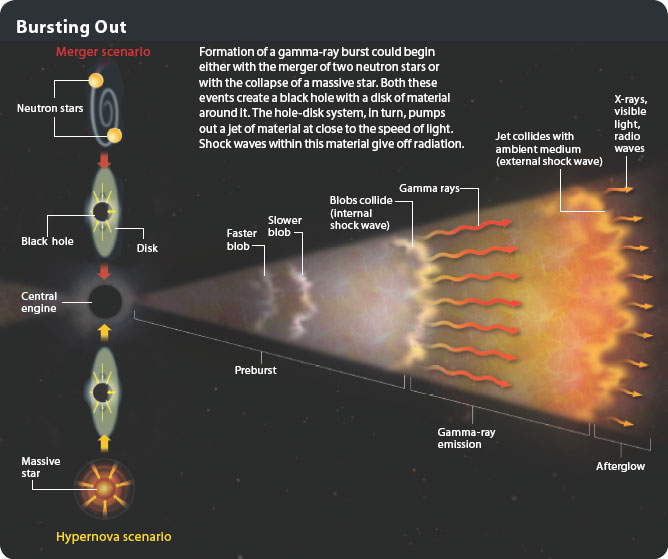
\includegraphics[scale=0.5]{Figures/fig5.png}
\caption{Visualisation of the fireball model (from Gehrels et al. (2002), credit
Juan Velasco)\citep{13}}
\end{center}
\end{figure} 
The  emitted  energy  is  higher than  the  mass of  the baryon in the rest frame by a factor of  $\sim $ 100, with  the  baryon  accelerated  with in an expanding fireball to a higher Lorentz factor, $\Gamma $. During this process, two major out comes can be seen: at the photosphere, a fraction of the thermal energy is radiated away  and  the  accelerated  electrons  produce  a non-thermal  gamma ray spectrum by a synchrotron  or an IC  processes in the  internal shock at large jet radius. Rather, the outflows that form from the central engine are believed to be dominated by Poynting flux \citep{15}\citep{16}.\\\\
The shocks in the fireball model are collisionless, whereby the particles involved are accelerated and scattered within the Fermi process when crossing the shock interaction. This can result in the type of energy distribution that can be described by a power law ($ \alpha $  $ \sim $ 2 - 3). In such a situation, the electrons emit a non-thermal radiation of photons via two different mechanisms, synchrotron and Inverse compton scattering, that extend to very high energy (GeV bands). \citep{10} \citep{17}. 
\subsubsection{Disspative process}
Dispative process :- is the  of outflows or shock waves from central engine  interact with interstellar medium ( ISM ) to produse both GRBs and its afterglow - the external and internal shock models, that  successfully interpret the prompt and afterglow emissions respectively.In particular, the origin of the emissions associated with the two phases is produced by two different processes. \citep{8} \citep{17}.\\\\
\textbf{Internal shock model}\\
The internal shocks are the mechanism for the production of the observed highly energetic gamma-rays. Moments after the initial GRB event, shock waves emanate from the inner engine at relativistic speeds [99.995\%  of the speed of light at a Lorentz factor of $ \sim 100 $. The fireball is dynamic; it isn't just one shock wave emanating from the compact source. Instead, different shock waves will  be traveling at different relativistic speeds, and it is the interaction between these different shock fronts that cause the energetic gamma-ray emissions \citep{17}\citep{18}.\\\\
The internal shocks traveling  at relativistic speeds  convert  kinetic energy into gamma-ray photons, this is  the only way to  get high  energy gamma-rays that are observed (as previously mentioned, they cannot be emitted through a thermal process). When  internal shocks interact with  each  other as they  are  moving  at  relativistic  speeds, the  interactions  produce  Inverse  Compton and Synchrotron emissions\citep{18} (see fig2.2).\\\\
\begin{figure}[h]
\begin{center}
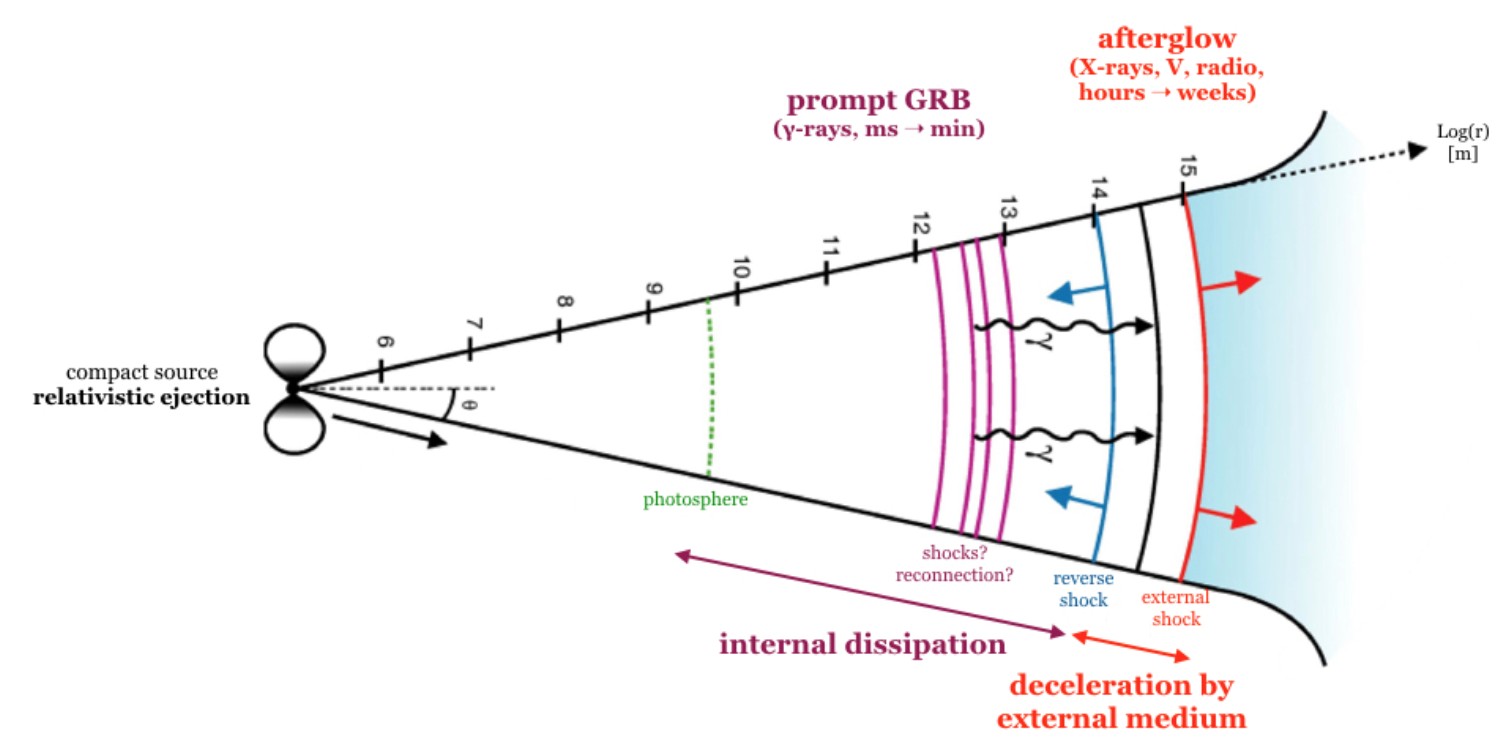
\includegraphics[scale=0.2]{Figures/fig6.png}
\caption{Standard fireball model.}
\end{center}
\end{figure}
Initially, the fireball is optically thick but as it expands and cools it becomes optically thin, allowing the gamma-ray photons to escape. Early models had the fireball and the internal shock waves as being purely radiative, but this didn't follow what was being observed (it would have made a profile too smooth). To solve this problem, some baryonic mass was added. This allowed for the internal shocks to become effectively contaminated. The added baryonic mass also aids in the conversion of some radiation energy into kinetic energy, which helps with an added kick to the relativistic kinetic energy of the shock waves, this in turn increases the gamma-ray energy more,Even if all of the shock waves emanate from the core at the same speed they will eventually cross over multiple times. As the shells are emitting through inverse Compton, it is slowing the shock front, thus increasing the times that many shock waves interact with one another. The earlier shock waves are likely to be emitted slower than the later emitted shock waves, this would also increase the amount of interactivity between the different shock waves.\citep{10}\citep{18}.\\\\
\textbf{External shock model}\\
The external shock waves are used to explain the afterglow that was first detected by BeppoSAX in 1997, as the internal shock waves are not able to explain the duration of the afterglow nor the wavelengths that are detected (which range from soft x-ray through to radio). The name can be a little misleading at first; the external waves actually refer to the internal waves at a later stage --once they've cooled down and continue emanating from the source. As the shock waves continue out they will eventually interact with the Interstellar Medium [ISM] (such as a molecular cloud or some other impedance), and it is the shock waves' interaction with the dust/gas that cause the afterglow . Unlike the internal shocks, the external shocks are primarily a thermal emission(see fig 2.3). The energy transferred from the shock waves is deposited into the ISM; this material can then be caught up in the shock front and emit radiation. As the shock waves began with a lot of energy, there is a lot that can be deposited into the ISM, this is what can cause such long afterglow and why it covers all parts of the energy spectrum \citep{19}.\\\\
\begin{figure}[h]
\begin{center}
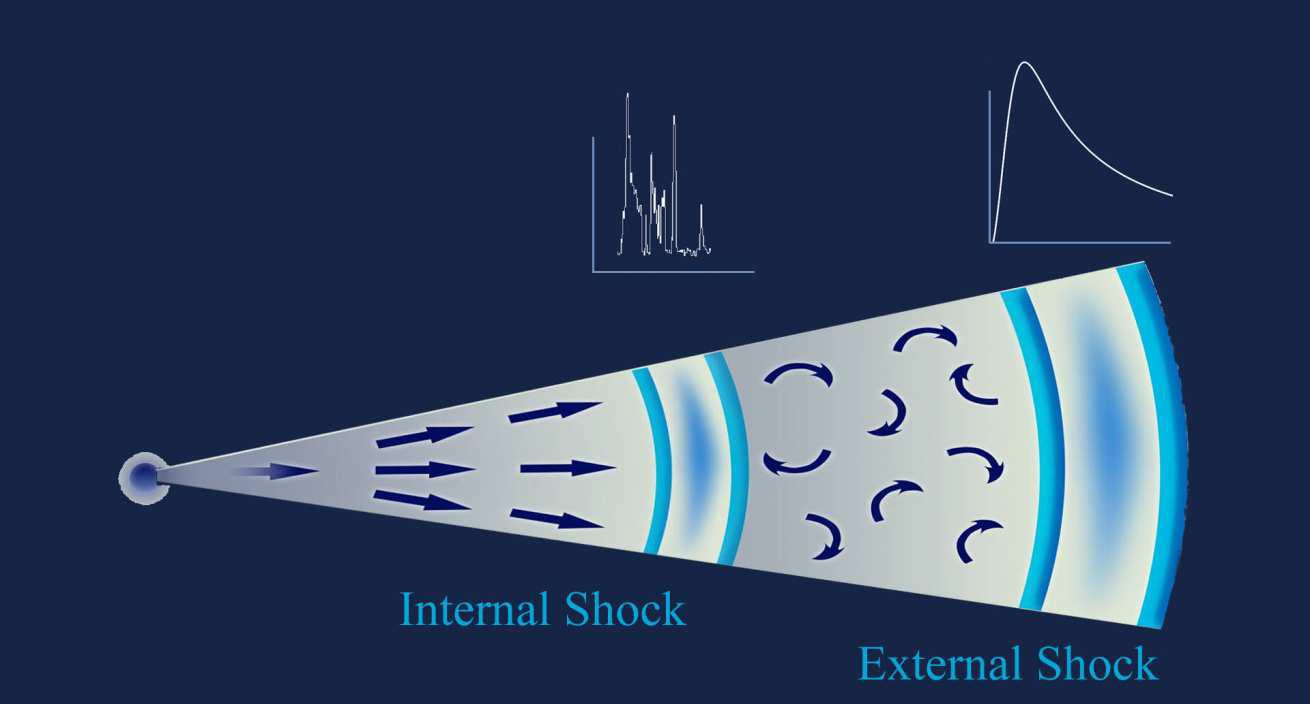
\includegraphics[scale=0.3]{Figures/fig7.png}
\caption{Qualitative schematic view of the structure of the relativistic jet produced by the gamma-ray burst. The external
shock arises as a result of the impact of the jet on the stellar wind of the progenitor. This is where the final goodbye of the SOS
similar emission from the collapsing star forms, which is characterized by a smooth (but non-monotonic) light variation. The
internal shock persists as long as the central engine continues operating this is where rapidly varying gamma-, x-ray, and
optical radiation forms.}
\end{center}
\end{figure}
A relativistic materials/jets are running into some external ambient medium i.e in-
terstellar medium or stellar wind. In each time, the ejecta run a high density envi-
ronment in which they produced a peak in the mission called external shock [38]. In
the external shocks, the jets may be forward shocked or reverse shocked.As the material in the jet expands, accelerates and compresses interstellar medium,It creates a forward shocks. The deceleration of forward shocks is occurred when the rest mass energy of the swept up particles equal to the ejected energy. This sets a deceleration length scale at ($\sim  10^{16} $ cm) . The reverse shock is formed by the deceleration of the jet material and propagates back into the relativistic flow. This happens when the rest mass energy of the swept up particles is greater than the ejected energy \citep{20}.\\\\
Although it would be correct to assume that all GRBs have an external shock, about half of detected GRBs don't have a detectable afterglow. The reason that no afterglow is being detected is not thought to be because the exposures aren't long enough, or because we're observing too early or too late. Rather, GRBs occur in high mass systems, whether it be through a supernova or NS-NS and NS-BH merges, this means that they've had very short stellar lives and may still be inside of a molecular cloud. Molecular clouds are very optically thick environments so the reason we're not able to detect the afterglow in about 50\%  of the time could just be due to reddening, absorption, or scattering.
\subsubsection{Radiative process}
\textbf{ Synchrotron Radiation}\\
Synchrotron emission is the non-thermal radiation produced when a relativistic
electron gyrates in a uniform magnetic field. Synchrotron radiation can explain
the GRB prompt emissions, and is considered to be one of the more important
mechanisms in various astrophysical phenomena. The synchrotron shock mechanism,
which is produced by the optically thin plasma in a weak magnetic field, can be
used to predict the form of the observed spectra \citep{1}\citep{15}\citep{18}\\\\
Synchrotron emission can be classified as having two regimes: the "fast-cooling"
phase,which describes when the timescale for the cooling of the electrons is shorter
than the dynamical lifetime of the source, resulting in an electron that cools quickly compared to the low-level injection of energy; conversely, "slow-cooling" occurs when the timescale for the cooling of the electrons is longer than the dynamical lifetime of the source . The differences between these two regimes are associated with the emission’s radiative timescale \citep{9} \citep{10}.\\\\
The peak frequency, the cooling frequency, and the self-absorption frequencies set
the characteristic break frequencies in the synchrotron spectra. These frequencies
evolve with time;indeed, their evolution is reflected in the complexities observed in
the shapes of the light curves at certain band energies . This model can successfully
describe the afterglow. Thus, the optically thin synchrotron spectrum is currently
considered the best spectral fitting model for most GRBs. The first synchrotron
model was applied to the spectral fitting of GRBs by Tavani (1996), and subsequently
by Baring and Braby(2004)\citep{15}\citep{16}.\\\\
\textbf{Synchrotron Self-Compton}\\
Inelastic collisions between low-energy photons and ultra-relativistic electrons are
known as the IC processes. Each astrophysical source has an Synchrotron Self-
Compton (SSC) scattering component when synchrotron radiation that energizes
it provides the means to scatter its seed photons to high energies and across a large
frequency range. Thus, the phenomenon responsible for creating high-energy emissionsfrom GRBs and other astrophysical sources is accepted to be the SSC mechanism. The SSC mechanism, while complex, uses a simple power-law function to explain the injected electron spectrum. The SSC spectrum can be described precisely as carrying out a complicated seed photon spectrum convolution and electron energy distribution. In certain circumstances, the GRB spectrum can be modelled as an SSC component at very high energy $ \sim $10 MeV.\citep{11}\citep{16} 
\subsection{ progenitors of GRBs}
\subsection{Working mechanisms of centeral engine}
The inner engine is of great importance, as it needs to be able to push material out very near the speed of light. The inner engine of a GRB is a highly compact source, and it is the highly compact nature of this object that leads to the idea that the core of the inner engine of a GRB is either a neutron star or a black hole (as they're the two most compact sources that we're currently aware of )
The workings of this inner engine will alter depending on whether it is a long or short GRB being observed. A short GRB has been theorised as occurring during a neutron star binary collision [NS-NS] or a neutron star-black hole collision [NS-BH]. It has been suggested that a long GRB could be associated with a hypernova -- a Wolf-Rayet type star undergoing a core collapse supernova.\citep{21}
\subsection{GRB-SN assocition}
\section{GRBs Obsevations and interpretations }
GRBs composed of two main radiative phases: the prompt and aferglow phases.The
former typically observed in soft gamma-ray (10 keV to 10 MeV), and generally
lasts between $ \sim $ 100ms and $ \sim $ 1000 s, although there is a wide variety of different temporal behaviors observed,from single pulses to complex temporal evolution. The spectrum of this prompt emission is non -thermal, often described by a Band function with a typical peak around $ \sim $ 200 keV.
The afterglow emission is most often detected from X-rays to radio waves and fades
with time. In the optical, the temporal fading goes typically as $ t^{-1} $ , however the slope of this fading depends on the wavelength and on the burst. This means an
afterglow observed in the optical will frequently fade beyond the reach of most
ground-based telescopes within a week. In the radio however, there is evidence of
emission from the afterglow up to a few months or even years after the burst.
The sudden flash of gamma rays emitted in the creation of a GRB was the route
by which GRBs were detected and the property for which they are named. The
prompt emission is readily detected, even by rudimentary space-based gamma-
ray detectors, due to the extreme high-energy photon budget that GRBs exhibit.
Indeed, at peak, GRBs outshine all other sources within gamma-ray sky, including
the Sun.\citep{18}\\\\
\subsection{ prompt GRB emission}
 prompt emission of GRBs is defined as the emission observed during the gamma-/hard X-rays phase, whose photons are the ones triggering the space instrumentation leading to multi-wavelength follow-up observations.	It is believed to be the direct outflow ejected from the central engine; as per the "fireball" model,which deposits its gravitational energy into a thermal explosion. In other words, the prompt emission occurs when the kinetic energy from a catastrophic explosion event, such as massive star core collapse or the merger of two compact stars, is converted into electromagnetic radiation due to the internal shocks that result from collisions between shells of ejecta.\citep{23}\\\\
prompt emission generated due to internal shocks magnetic dissipation within the
fireball take place effectively above the pair production photosphere at $ 10^{12} $ to  $ 10^{14} $ cm.These shocks splits from mini-shells within a jet produced by unsteady accretion of materials onto black hole or by the merger of binary neutron stars (BNS). The shells have a distribution in lorentz factor $ \gamma $ $ \propto $ $ \Gamma $ where $ \Gamma $ is bulk lorentz factor.\citep {22}\citep{23}\\\\
\begin{figure}[hpbt]
\subfloat[]{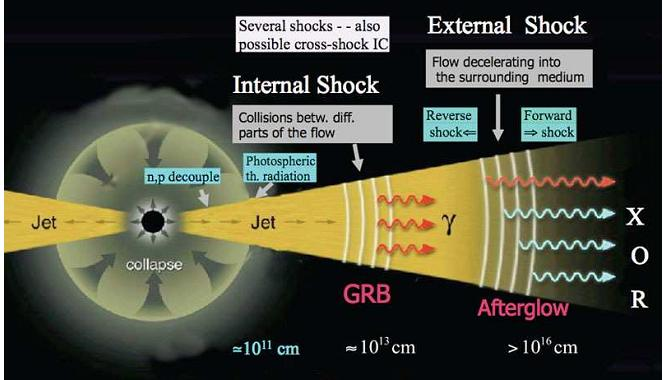
\includegraphics[scale=0.4]{Figures/collapser.png}}
\subfloat[]{\includegraphics[scale=0.4]{Figures/fireball.png}}
\caption{Schematic evolution of the jet Lorentz factor and examples of symbolic locations of radius: the saturation radius $r_{s} $ , photospheric radius $r_{ph} $ , internal shock radius $ r_{is} $ and external shock $ r_{_{es}} $}
\label{GRB prompt emission}
\end{figure}
In the region around $ \sim $ $ 10^{12} $ cm to  $ 10^{14} $ cm , the collisions between different parts of the flow is produced in different shells (see fig 2.4 (a) and(b)). As a fast shell catch up with a slower ones, they form strong internal shocks that propagates in both shells with out deceleration. Once shell became above the photosphere,the heated and accelerated electrons cool by synchrotron emission then radiation is observed in $ \gamma $-ray band. Each collision that occurs above pair photosphere produces a pulse in the GRB’s light curves\citep{22}\\\\
Thus, GRB light curves represent the count rates/photons recorded by the
high energy detectors as a function of time. Each of the recorded events shows
different variability patterns, meaning that each light curve is different from the
rest. As it is shown in Figure 2.5, the light curves can be classified into four
different categories Pe’er, 2015:\\
• single-peak events (e.g. GRB 910711),\\
• a smoothed light curve composed with several peaks (e.g. GRB 920221),\\
• separated multi-collisions (e.g. GRB 930131A),\\
• and irregular peaks (e.g. GRB 991216)\\
\begin{figure}[h]
\begin{center}
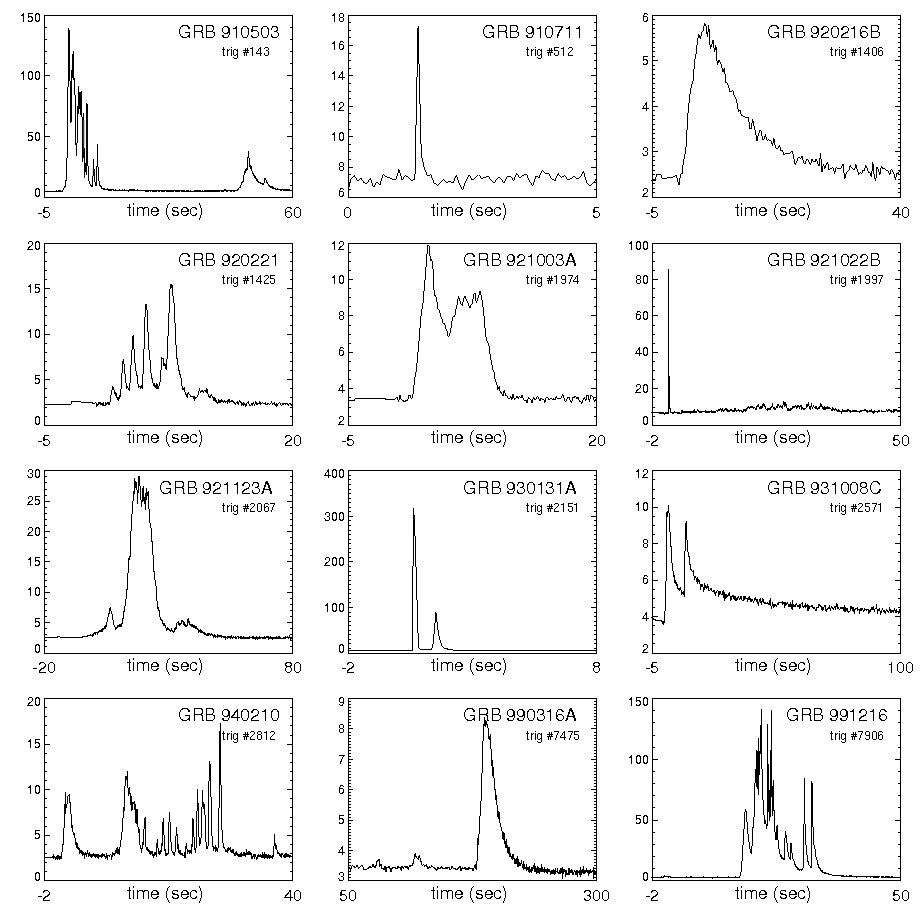
\includegraphics[scale=0.4]{Figures/prompt.png}
\caption{Diverse light curves of the GRBs prompt emission detected by BATSE instrument.This sample includes short and long events. https://gammaray.nsstc.nasa.gov/batse/grb/lightcurve/}[Firaol Fana]
\end{center}
\end{figure}
The result is that the fireball expands due to the effects of thermal pressure and
is then accelerated to relativistic speeds, where the thermal energy is ultimately
released in the form of photons at the photosphere. In the internal shock case,
the dissipation happens inside the ejecta, where the ejecta is decelerated by the
surrounding medium and this deceleration happens after the internal shock phase
ceased. \citep{6}\citep{10}\citep{23}
\subsection{Afterglow GRB emission}
Afterglow is the phase of GRBs that slowly fading at longer wavelength. This
emission is created by the collision between ejected bursts and the surronding
medium or interstellar gas or dust. The GRB itself is rapid, lasting from less than a second up to a few minute at most. Once it disappears, it leaves behind a counterpart
at a longer wavelengths from X-ray to radio bands . Then, they are remain
detectable for days or longer. As we have mentioned above, afterglow emissions are
dominated by external shocks.Due to luck of advanced instrument, early searches
were unsuccessful largely to observe the bursts’ position at a longer wavelength
immediately after the initial burst,Once the GRB faded deep imaging was able to
identify a faint, distance host of galaxy at a location of GRB as pinpointed by the
optical afterglow.\citep{15}\citep{22}\citep{23} 
\section{Interpretations of afterglow GRBs}
Before launch of the Swift satellite, broad-band, late time (t > $ \sim $ 10 hours) afterglow data had been collected for a moderate sample of GRBs. These observations were generally consistent with predictions of the external forward shock,synchrotron emission, model. The main observational properties of late time afterglow radiations are:\\
• In general the optical afterglow displays a power law decay behavior $ F_{\nu} $ $ \propto $ $ t^{-\alpha} $   , with a decay index $ \alpha \sim $ 1. This is consistent with the prediction of the standard external shock afterglow model.\\
• A temporal break in the optical afterglow light curve is usually detected for bright GRBs. The break time is typically around a day or so, which is followed by a steeper decay with slope $ \alpha  \sim $ 2. This is consistent with the theoretical prediction of a “jet break”.\\
• The radio afterglow light curve initially rises and reaches a peak around
10 days, after which it starts to decline (e.g. Frail et al., 2000). The peak
usually corresponds to passage of the synchrotron injection frequency $ \nu_{m} $ ,
or the synchrotron self-absorption frequency $ \nu_{a} $ , through the radio band.\\
• The broad-band afterglow spectrum can be fit with a broken power law, at
a fixed observer time as one expects for the synchrotron afterglow model.\\
• For bursts with high-quality data richer features in the optical light curves have been discovered, which include bumps and wiggles that deviate from the simple afterglow model predictions. Smooth bumps in afterglow lightcurves with duration $ \delta  t _{obs}  \sim  t_{obs} $ may be interpreted as due to density bumps in the external medium  where as sharper features in lightcurves might be due to energy injection from the central engine  angular fluctuations in energy per unit solid angle \citep{18}.
\subsection{Early time afterglow}
\subsection{Late time afterglow }
Before swift mission, afterglow observations was started after several hours (and 10 hrs) after bursts trigger. The optical afterglow of late time afterglow displays a power law decay behavior $ F_{\nu}   \propto   t^{-\alpha} $  , with a decay index  $\alpha  \sim  1 $ . The temporal break in the optical afterglow light curve was detected for bright GRBs. The break time is typically around a day and followed by the steeper decay with decay slope of $ \alpha  \sim 2 $ \citep{24}\\\\
The radio afterglow light curve initially rises and reaches a peak around 10 days
after which starts to decline . The peak usually corresponds to the passage of synchrotron injection frequency $ \nu_{m} $ or synchrotron self absorption frequency $ \nu_{a} $through the radio band. The broad band afterglow spectrum can be fit with a broken power law at a fixed observer time.\citep{25}
\section{Theoritical interpretation of X-ray afterglow}
Afterglow GRBs  observed at all wavelengths such as: X-ray \citep{26}, optical \citep{27}, IR, and radio \citep{28}. Thanks to its low variability and observed time range (from minutes to weeks after the GRB event), a canonical X-ray light-curve for the afterglow was defined from the result of Swift /BAT-XRT instruments. (It is displayed on Fig2.5 ). From the fig , the 0 symbol indicates the prompt phase, and the four remaining segments, with their corresponding temporal indexes, are associated two by two and identified as early and late afterglow \citep{29},\citep{30}\citep{31} : I and II (respectively the steep and shallow decay), and III and IV (respectively a standard afterglow and a jet break). Part I and III, marked by solid lines, are most common and the other three components, marked by dashed lines, are only observed in a fraction of all bursts. Part I, thought to be associated with the prompt phase  when the central engine is still active; the rest of the afterglows are due to the dynamics of the interaction between the jet and the surrounding medium.\citep{6}\cite {15}\citep{18} \citep{32}.\\\\
\begin{figure}[hpbt]
\subfloat[]{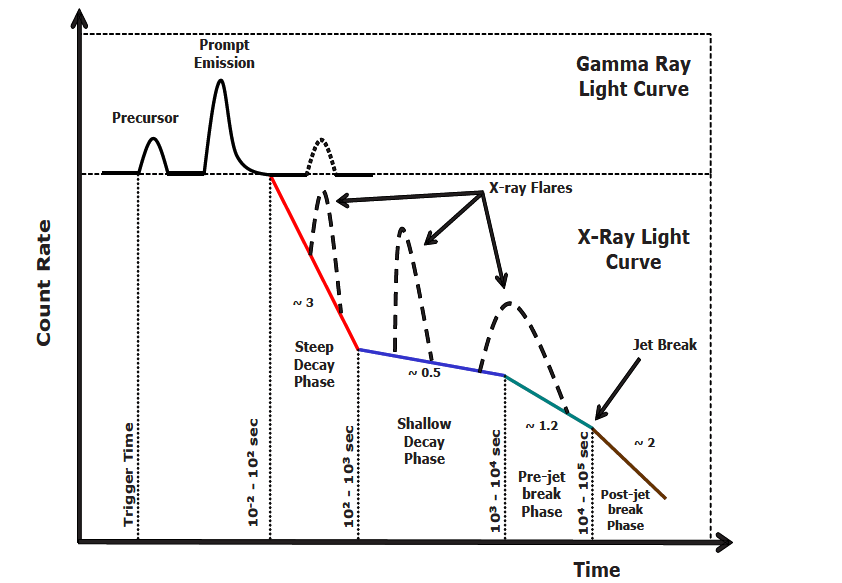
\includegraphics[scale=0.3]{Figures/X-ray Lc.png}}
\subfloat[]{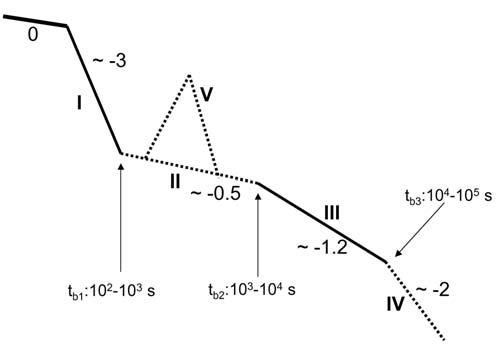
\includegraphics[scale=0.4]{Figures/Lightcurve.png}}
\caption{Canonical GRB light curve. The prompt phase is often followed by a steep
decay phase (typical index of 3) which can then break to a shallower decline (shallow decay phase), a standard afterglow phase (pre-jet break phase), and possibly, a jet break and post-jet break phase. Sometimes an X-ray flare is seen.}
\label{Fg: Theoritical interpretation of X-ray afterglow}
\end{figure}
The detection of GRBs early afterglows is within less than 100 seconds after trigger
in the swift mission. The canonical X-ray afterglow light curve generally includes
four phases such as early time steep decay phase, the shallow decay /plateau
phase, normal decay phase and late steep decay phase \citep{33}.\\\\
\subsection{steep decay of early X-ray light curves}.
This phase is the tail of prompt emission that governed by curvature
effect, for which emission from different viewing angles reaches the observer with
different delays due to the light propagation effects \citep{33}. The relationship between temporal and spectral slopes of higher latitude emission is $\alpha  = 2 + \beta $. It is independent of any of the environmental or other parameters such as peak frequency and cooling frequency that affects the closure relations for the external shocks.\\
Swift answer the debate of separation between the prompt emission and late af-
terglow regarding to internal and external origin of the prompt emission i.e internal
shocks are the origin of prompt emission \citep{33}. As it has shown in (Fig2.6 above ), slope of early steep decay is around $3 < \alpha_{1} < 5$.
This phase may be simply the high latitude emission associated with the prompt
gamma-ray sources at $ R \gtrsim 10^{15} $ cm when the central engine turns off faster than the decline of the X-ray light curves . On the other hand, if the emission region is at much smaller radius than the rapidly declining X-ray light curve reflects the time dependence of central engine activity\citep{36}.\\
Detailed analysis of a sample of GRBs suggests that the high latitude ”curvature
effect” model can explain the early steep decay phase \citep{37}. As we have shown in
(Fig 2.5), the achromatic change of phases for sample GRBs indicates the light
curves transition. These GRBs followed the decay power law relation $ F_{\nu}\propto  t^{-\alpha_{1}} $ where, $ \alpha_{1}  = 2 + \beta $ for curvature effect model. Generally, this phase has already stayed between the time interval of $ 10^{-2}  - 10^{2} $ seconds and $ 10^{2} - 10^{3} $ seconds that  presented (in fig 2.6) at the right side.\\\ 
\subsection{Shallow /plateau decay X-ray light curves }
This phase is sometimes called plateau phase and very small decay with value of decay
$0.5 < \alpha_{2} < 1.0 $. This phase rises when the energy ejected to the decelerated external shock. When the energy is terminated, the decay of light curves become slow down and the transition to phase three (normal decay) is occurred [51]. In this phase, the shape of light curves in the X-ray and optical bands should be similar where break occur at the same time in these bands.\citep{38}\citep{39} .\\\\
There are two acceptable explanations behind the emission mechanisms of this
phase. (1) A smooth and gradual energy injection that arrives in the forward shock,
is due to the decrease of the lorentz factor $ \Gamma $ at the end of prompt emission. The mass that is injected to the forward shock is the function of its lorentz factor and the energy injected. As a result $ \Gamma $ increases monotonically with radius,(which we discussed in detail in section (2.6). The flux decays are a power law and depends on the mass and the energy injected . (2) The central engine of the source stays active for hours after the burst and injects the smooth and continues energy at later times, several times after the burst\citep{40} \citep{41}.\\
X-ray plateaus results from the contribution of prompt X-ray emission scattered
by dust in the host galaxy. The optical flux or the powerful outburst episode is
already ruled out by the prompt optical data\citep{42}.\\
\subsection{normal decay phase}
This is the third phase in this canonical phase description. This phase has a decay
slope around $1.0 < \alpha_{3} < 1.5$ which was expected before swift and it is consistent standard fireball afterglow model in ISM [56]. The explanation of this phase is related to the end of energy injection at the external shocks.
This implies (1) the fall of the lorentz factor of forward shock up to the point of
minimal lorentz factor that carries a significant initial energy. (2) The time that the central engine needs to be in active. In general the normal decay is expected in the standard forward shock.\citep{43}
\subsection{Late steep decay following the plateau in X-ray light curves}
 The early steep decay represented at the left side of fig 2.6 , the decay slope is greater than 2. After the normal decay, X-ray emission is powered by a continues jet from a long lasting central engine. Then X-ray flux from the external shock is buried beneath this emission [58]. Indeed, the canonical X-ray light curve can be matched with the accretion history in the collapsar GRB model. This model assume that the X-ray luminosity is proportional to the accretion power of the central engine [59].
This late steep decay of swift, represents an achromatic steepening that happens
due to the jet breaks. When the lorentz factor of the ejecta becomes larger than
$ \theta_{0}^{-1} $ compared to the jet opening angle $ \theta_{0} $ , the ejecta is collimated into a jet break. Finally, this phase is expected in the forward shock model as a jet break. Jet breaks are thought to happen due to the beaming of the emission from GRBs. This phase has pre-jet-break phase and post-jet-break phase, (see in Fig 2.6).\citep{44} \citep{45}
\subsection{Time breaks in swift X-ray afterglow}
As shown in (Fig 2.6), there are three break points and the time at that points are called breaking time of afterglow light curves. These break times are the first break time, the second break time and the jet break time.\\
\subsection{The first break in the light curve ( $ t_{break,1} $ )}
This is the time at which the phase change of light curves from phase I to phase II is took places. As we have shown in (Fig2.6), the $ t_{break,1} $ is around  $t_{break,1} (10^{2} - 10^{3} ) $ s  < $ t_{1} $ <  $ t_{break,2}( 10^{3} - 10^{4})$ seconds).\\
The first break time is also the time when the slow decaying emission from the
forward shock become dominant over the rapidly decaying flux from the prompt
emission at a large angle. In sharply decaying flux, the prompt emission initially
dominates over the external shocks at t > $ t_{break,1} $\citep{46}.
\section{Decay of flux with time of observed light currve }
The fluence (S) is the total radiant energy collected from the GRBs per unit area over the duration of the event (i.e., $ T_{90} $ ). It is computed by integrating its energy flux over time and the energy range of the detector (i.e., the total energy collected per unit time and per unit area). The fluence measured between energies $ E_{min} $ and $ E_{max} $ is given by[Firaol Fana]
\begin{equation}
S= T_{90}\int_{min}^{max}E\frac{dN}{dE}dE
\end{equation}
The energy flux of a burst is defined
\begin{equation}
F=\int_{Emin}^{Emax}E\frac{dN}{dE}dE
\end{equation}
When relativistic, conical and optically thin source moving with a lorentz factor     $ \Gamma $ turns off abruptly, the flux declines rapidly with time [61]. In such type of source which is specified with spherical co-ordinate (r,$\theta $, $\varphi $ ), the source turned off at $ r =  R_{0} $. where r is the radius of the photo/jets, $ R_{0} $ is the radius of the observer and$ \theta $ is measured with respect to the line of sight to the observer.
\begin{figure}[h]
\begin{center}
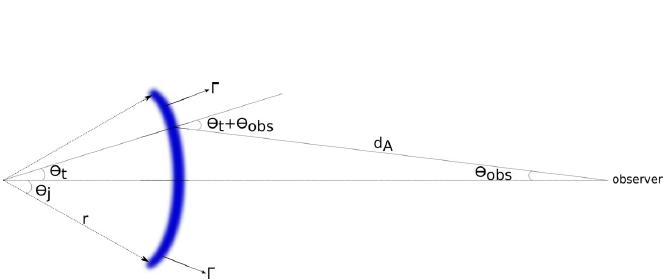
\includegraphics[scale=0.5]{Figures/Flux.png}
\caption{ A sketch of the various angles and distances for the large angle (or high
latitude) emission when the $\gamma$ -ray source turns off suddenly.}
\end{center}
\end{figure}
The time dependence of observed flux follows from the lorentz transformation of
specific intensity. The specific flux in the observer frame from the relativistic source of moving object with specific intensity $ I_{\nu'} $ and spectrum frequency $\propto $ $ \nu'_{-\beta} $ is given by
\begin{equation}
 f_{\nu}(t_{obs})= \int d\Omega_{obs} I_{\nu}cos\theta_{obs}
 \end{equation}
 where  $ d\Omega_{obs}$ is the solid angle of the source, $ I_{\nu} $  is the specific intensity of the source photon. To derive the standard flux decay of GRBs, let we define $ d\Omega_{obs}$   and $ I_{\nu} $ in the relativistic beaming.\\\\ In relativistic beam of photons, the transverse component of the momentum does not change under lorentz transformation,i.e its comoving and lab frame values are the same. Thus
\begin{equation}
\nu sin\theta = \nu'sin\theta'
\end{equation}
or
\begin{equation}
sin\theta =\frac{\nu'}{\nu}sin \theta'
\end{equation}
Since the photon frequency on the observer frame, $ \nu $, can be expressed in terms of the comoving frequency, $ \nu' $, using standard lorentz transformation of photon as
\begin{equation}
\nu =\frac{\nu'}{\Gamma (1 -\frac{\nu cos\theta}{c})} =\nu'D
\end{equation}
where $ D $ is standard doppler effect which is expressed as $ [\Gamma (1 -\frac{\upsilon cos\theta}{c} )]^{-1}$ . Then the ratio of the frequency become $ \frac{\nu'}{\nu} = \frac{1}{D}$ and substituting this ratio into Eq. (2.5), we obtain
\begin{equation}
sin\theta = \frac{sin\theta'}{D}
\end{equation}
For large $\Gamma$ , $\theta  \approx \frac{\theta'}{\Gamma}$. This tells us photons are focused in the forward direction
such that the angular size of photo beam in the lab frame is smaller than it is in the comoving frame by a factor $\sim \Gamma $. And also the solid angle for a canonical beam of
photons in lab frame is smaller than in the comoving frame by a factor of $\sim \Gamma^{2}$ . This implies the lorentz transformation of solid angle is
\begin{equation}
d\Omega =sin\theta d\theta d\phi =\frac{sin\theta'd\theta'd\phi'}{D^{2}}= \frac{d\Omega'}{D^{2}}
\end{equation}
The other parameter in the lorentz transformation is the specific intensity. It is
defined as flux per unit frequency and solid angle carried by photos traveling with in a narrow conical beam with its axis perpendicular to surface dA. This means
\begin{equation}
I_{\nu} =\frac{dE}{d\nu dt_{obs}dAd\Omega}
\end{equation}
Considering $ d\nu'dt'{obs}dA' $ = $ d\nu dt_{obs} dA $, are lorentz invariants and using Eq. (2.8) and $ E=\Gamma E' $ , Eq. (2.9) can be reduced to
\begin{equation}
I_{\nu} =D^{3}I'_{_{\nu'}}
\end{equation}
\section{calculating luminosity (L) of x-ray afterglow}
Luminosity is the total amount of electromagnetic energy radiated (out put) by an  object per unit of time. The observed isotropic-equivalent luminosity in the X-ray afterglow ,$ L_{x} $ can generally be expressed as 
\begin{equation}
L_{x}(t)= \int_{\nu_{1}}^{\nu_{2}} L_{\nu}(t)d\nu
\end{equation}
 where $ L_{\nu}(t)=\dfrac{4 \pi d_{L}^{2} F} {(1+z)} $,substituting  $L_{\nu}(t)$ in to equa. (2.4) reveals 
 \begin{equation}
 L_{x}(t)=\dfrac{4 \pi d_{L}^{2}} {(1+z)}\int_{\nu_{1}}^{\nu_{2}}\frac{F_{_{\nu}}}{(1+z)[(1+z)t]d\nu} 
 \end{equation}
where $ d_{L} $ is the luminosity distance, $\nu_{1}$  and $ \nu_{2} $ are the spectral frequencies in the energy band, z is the redshift and $ L_{\nu}  (t) $ is the spectral luminosity at the cosmological frame of the source, i.e, both $\nu $ and t are  measured in the frame [62].
